%-----------------------------------------------------------------------
%
%     This file is part of the Code_Saturne Kernel, element of the
%     Code_Saturne CFD tool.
%
%     Copyright (C) 1998-2010 EDF S.A., France
%
%     contact: saturne-support@edf.fr
%
%     The Code_Saturne Kernel is free software; you can redistribute it
%     and/or modify it under the terms of the GNU General Public License
%     as published by the Free Software Foundation; either version 2 of
%     the License, or (at your option) any later version.
%
%     The Code_Saturne Kernel is distributed in the hope that it will be
%     useful, but WITHOUT ANY WARRANTY; without even the implied warranty
%     of MERCHANTABILITY or FITNESS FOR A PARTICULAR PURPOSE.  See the
%     GNU General Public License for more details.
%
%     You should have received a copy of the GNU General Public License
%     along with the Code_Saturne Kernel; if not, write to the
%     Free Software Foundation, Inc.,
%     51 Franklin St, Fifth Floor,
%     Boston, MA  02110-1301  USA
%
%-----------------------------------------------------------------------
\section{SOLUTION FOR CASE 4}
This case is similar to case 3, with the following differences:\\
\hspace*{1cm}$\bullet\ $parallel computation on 2 processors\\
\hspace*{1cm}$\bullet\ $head loss\\
\hspace*{1cm}$\bullet\ $calculation of a spatial average\\
\hspace*{1cm}$\bullet\ $dealing with a user results file

The head loss is defined in the Graphical User Interface. Go to {\itshape Volume regions definition} under the heading {\itshape Volume conditions}. Click on ``Add'', unselect ``Initialization'' and select ``Head losses'' in the box named {\itshape Nature}. In the box named {\itshape Label}, name the head loss region. Define the limits of the head losses region in {\itshape Selection criteria}. The associated character string to enter is as foolows:
``$0.2 <= X$ and $0.4 >= X$ and $-0.75 <= Y$ and $-0.25 >= Y$''

\begin{figure}[h!]
\begin{center}
\begin{tabular}{c}
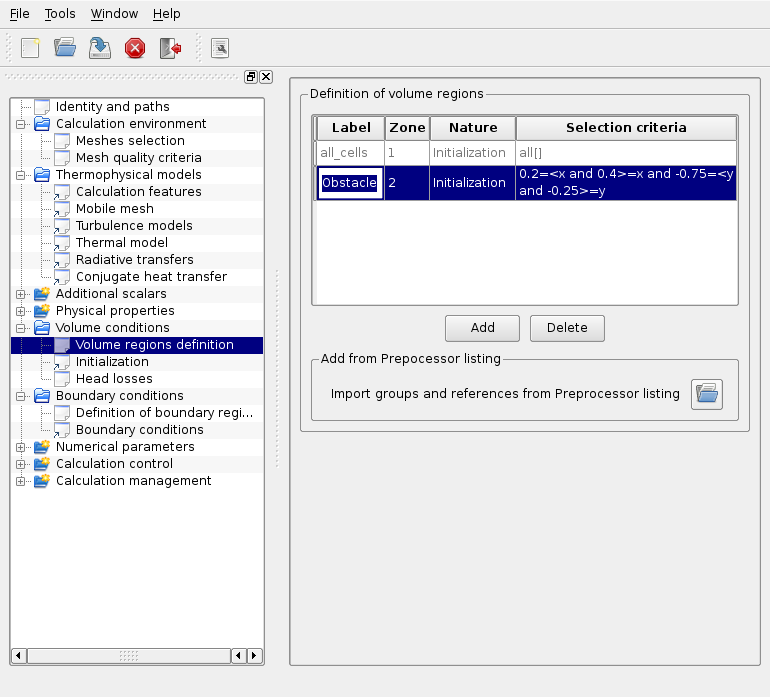
\includegraphics[width=9cm]{head_loss0} \\
\\
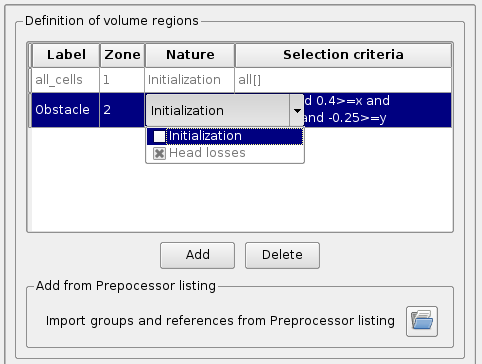
\includegraphics[width=9cm]{head_loss3}
\end{tabular}
\caption{Creation of head losses region}
\label{fig_hl1}
\end{center}
\end{figure}

\newpage
To specify the head losses coefficients go to the item {\itshape Head losses} and select the name of the head losses volume region. In this example, the coefficient is isotropic so that we use the same value for each $\alpha_{ii}$. Please note that $\alpha_{ii}=2 \times K_{ii}$, therefore if $K_{ii}=10^4$, $\alpha_{ii}=2 \ 10^4$.

\begin{figure}[h!]
\begin{center}
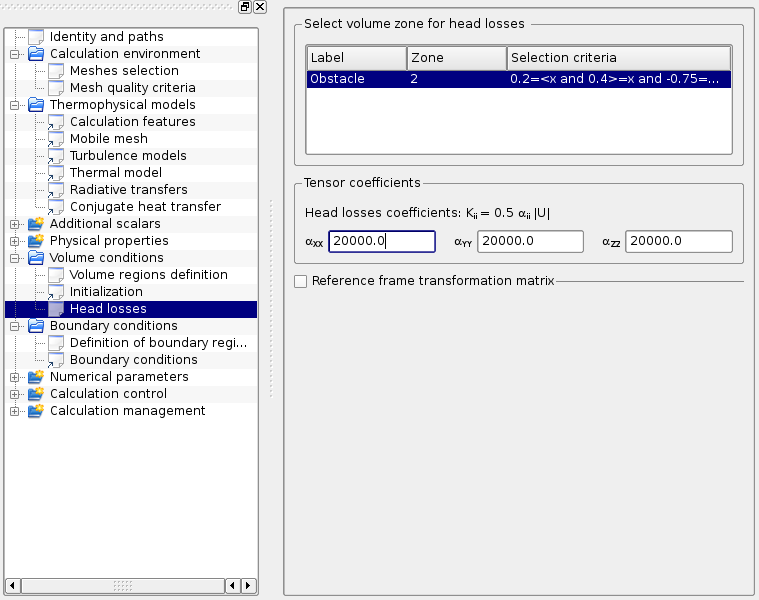
\includegraphics[width=12cm]{head_loss5}
\caption{Head losses coefficients}
\label{fig_hl2}
\end{center}
\end{figure}

\newpage
The calculation of the spatial average is done in the {\itshape usproj.f90}
routine. Refer to the example file in the
directory \texttt{examples} for the complete {\itshape usproj.f90} file.

The other two changes are controlled in the item
{\itshape Prepare batch analysis}.

To run the calculation on two processors, simply change the number of processors
indicator to 2. The launch script will automatically deal with the rest.

\begin{figure}[h!]
\begin{center}
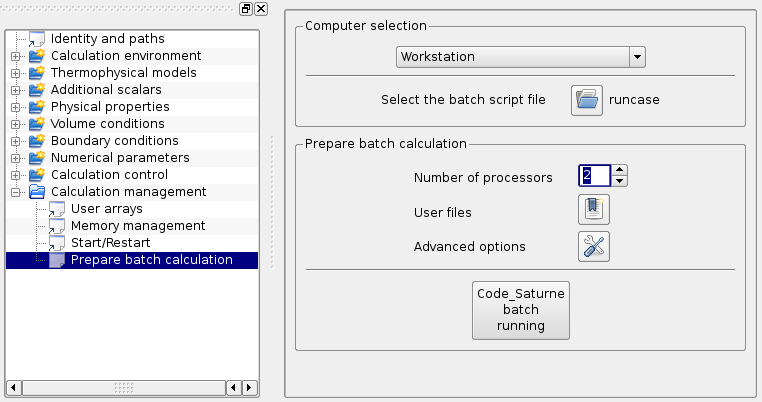
\includegraphics[width=12cm]{V-66}
\caption{Number of processors}
\label{fig1_e4}
\end{center}
\end{figure}


\newpage
As seen in paragraph \ref{prg_case4}, the file ``moy.dat'' created by
{\itshape usproj.f90} will be written in the temporary execution directory. It
must be identified in the launch script in order to be automatically copied in
the RESU directory (More precisely, a RES\_USERS.xxxxxxxx directory will be
created in the RESU folder, in which the file will be copied).

Click on the icon {\itshape New user result file} to enter the associated dialog window.
Enter the file name ``moy.dat'' in the field. Further file names can be added. When finished,
click on {\itshape OK}.

\begin{figure}[h!]
\begin{center}
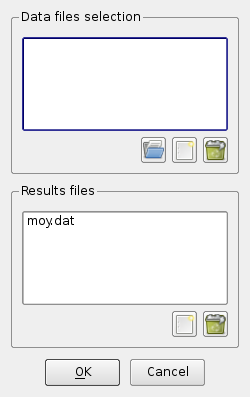
\includegraphics[width=5cm]{V-67}
\caption{User results files}
\label{fig2_e4}
\end{center}
\end{figure}


